\chapter{Progettazione e Implementazione} %\label{1cap:spinta_laterale}
% [titolo ridotto se non ci dovesse stare] {titolo completo}
%

\begin{citazione}
Vero cuore della tesi, in questo capitolo vengono analizzate nel dettaglio la progettazione e l'implementazione dei due diversi moduli sviluppati. Sebbene presentino caratteristiche comuni, questi vengono trattati in due diversi paragrafi, ciascuno pienamente dedicato alle scelte implementative del modulo d'interesse.
\end{citazione}

\section{Introduzione}
Pur condividendo le stesse finalità, i due moduli implementati presentano caratteristiche ben distinte tra loro. La scelta di tale distinzione deriva in primis dalla volontà di cimentarsi nello sviluppo di un'applicazione che consentisse a un giocatore di fronteggiare una CPU più o meno competitiva in una partita. In secundis, l'analisi delle prestazioni derivante dalla suddetta applicazione avrebbe poi spinto al confronto di diversi motori scacchistici, al fine di fornirne un'analisi delle prestazioni sempre più accurata e approfondita.

\subsection{Primo Modulo}
L'applicazione è stata realizzata in linguaggio Python. Come anticipato nel paragrafo precedente, l'intenzione è stata quella di sviluppare un'applicazione usabile da un utente umano per giocare una partita contro un'Intelligenza Artificiale: si è dunque ritenuta opportuna la progettazione di un'interfaccia grafica per l'interazione uomo-macchina. Attraverso la libreria \textit{pygame} è stato possibile creare l'interfaccia in modo programmatico, rappresentando le caselle con array di array di dimensione 8x8 e sfruttando semplici metodi per caricare le immagini dei pezzi precedentemente salvate nella cartella di lavoro. Inoltre, assieme ai pezzi, sono state distinte in maniera visivamente chiara e precisa le caselle chiare da quelle scure. 
\begin{figure}[!htb]
    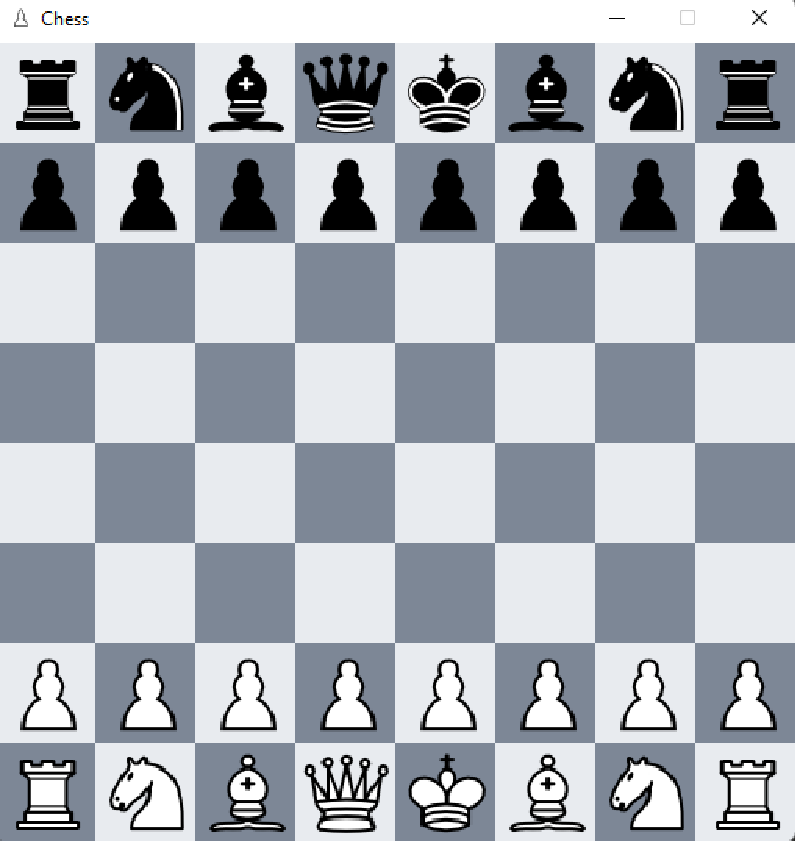
\includegraphics[width=10cm]{frontmatter/figure/scacchiera_gui.pdf}
    \centering
    \caption{Interfaccia grafica vista dall'utente}
    \label{fig:scacchiera_gui}
\end{figure}
\begin{figure}[!htb]
    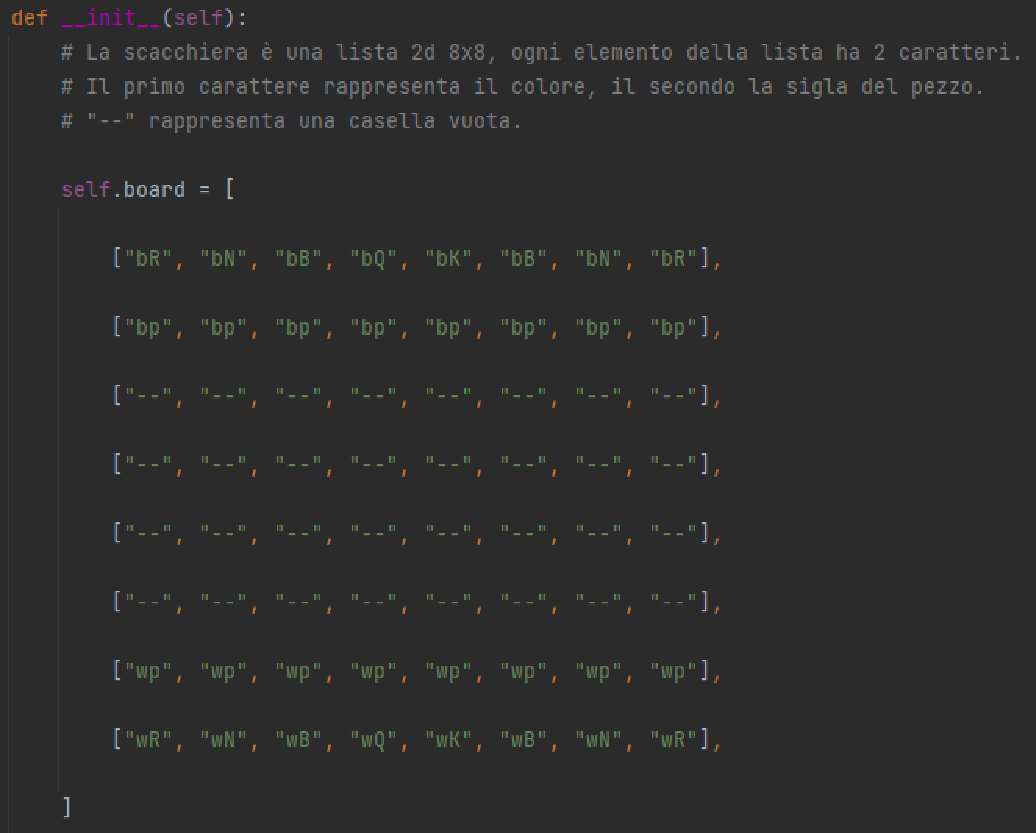
\includegraphics[width=10cm]{frontmatter/figure/rappresentazione_scacchiera.pdf}
    \centering
    \caption{Codifica della figura 3.1}
    \label{fig:rappresentazione_scacchiera}
\end{figure}
\newpage
% Per affiancare due figure
% \begin{figure}[!htb]
% \begin{minipage}[b]{7cm}
% \centering
% 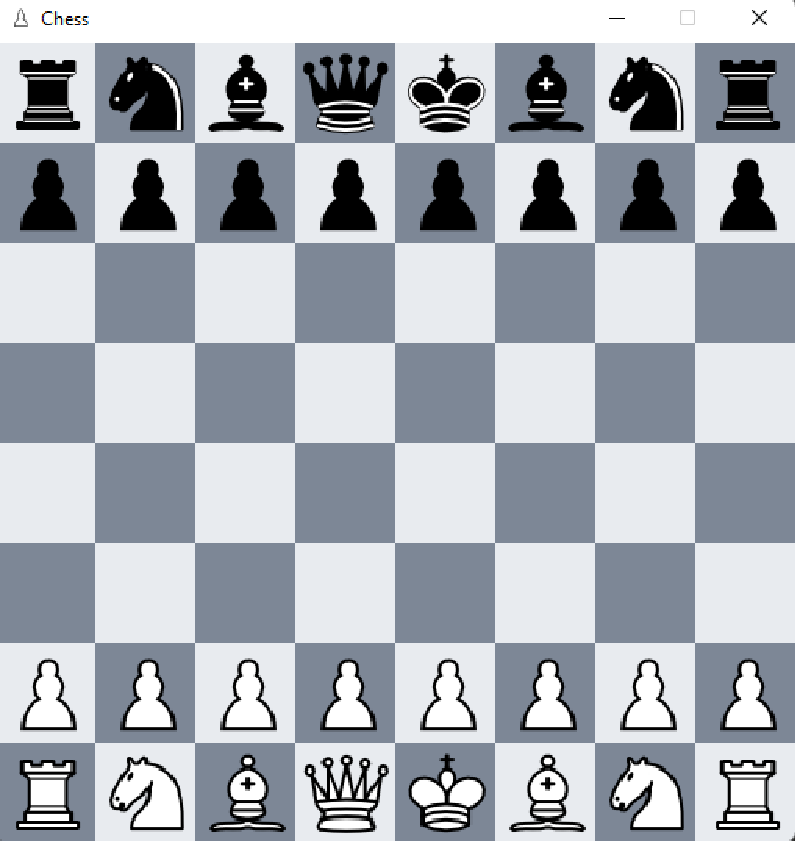
\includegraphics[width=6.5cm]{frontmatter/figure/scacchiera_gui}\\
% \caption{Interfaccia grafica vista dall'utente}
% \label{fig:scacchiera_gui}
% \end{minipage}
% \hspace{1mm}
% \begin{minipage}[b]{7cm}
% \centering
% 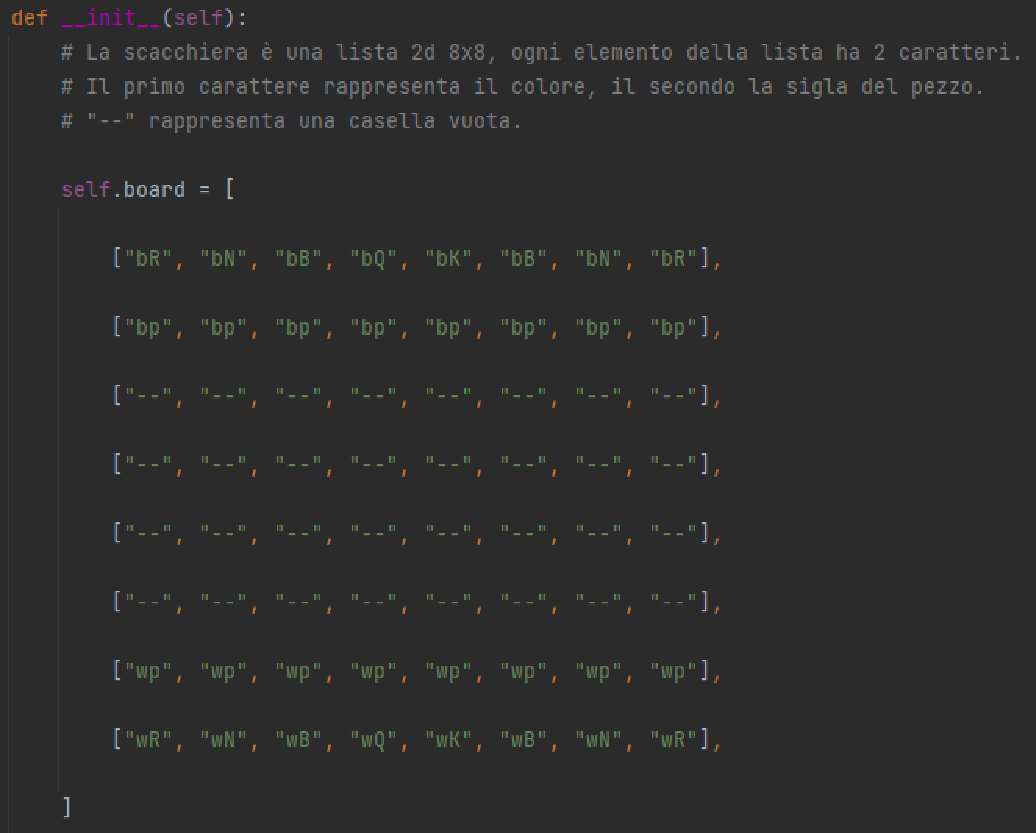
\includegraphics[width=8cm]{frontmatter/figure/rappresentazione_scacchiera}\\
% \caption{Codifica della figura 3.1}
% \label{fig:rappresentazione_scacchiera}
% \end{minipage}
% \end{figure}

A seguito della rappresentazione iniziale della scacchiera sono stati programmati i metodi che si occupano della generazione delle mosse possibili per ciascun pezzo, per impedire all'utente di effettuare mosse non legali\footnote{Nel gioco degli scacchi il pedone si muove in avanti di una casella (due per la sua prima mossa) e cattura di una casella in diagonale, la torre in orizzontale, l'alfiere in diagonale, il cavallo a L, la regina in orizzontale e in diagonale, e il re di una casella in tutte le direzioni.}. Analogamente, ad ogni mossa giocata viene effettuato un controllo nel caso in cui il re sia sotto scacco o nel caso in cui vi sia una situazione di scacco matto, dichiarando partita finita nel secondo caso.
\begin{figure}[!htb]
    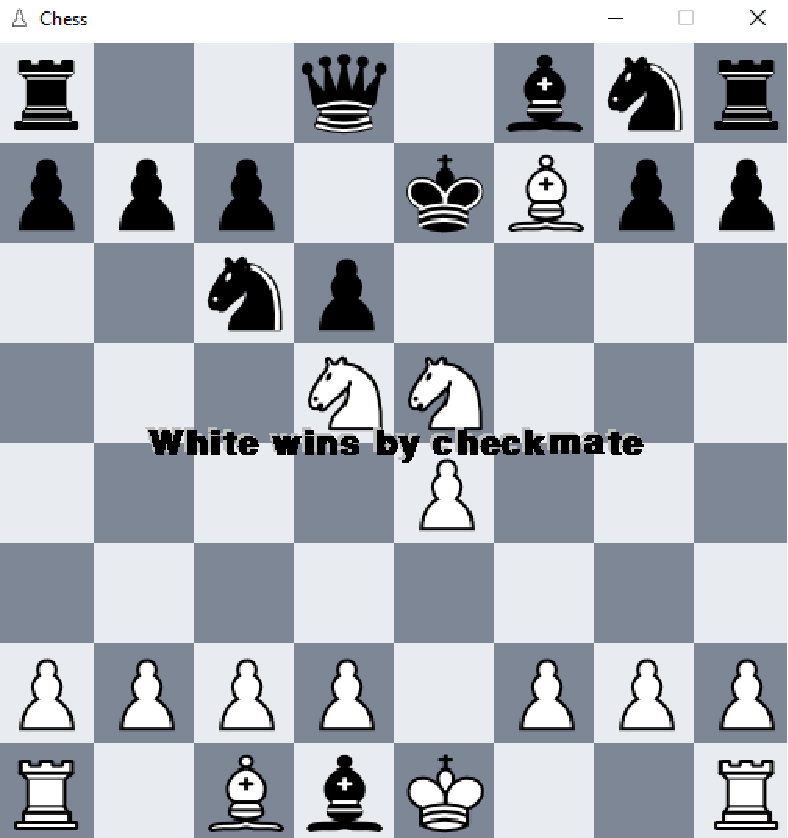
\includegraphics[width=10cm]{frontmatter/figure/checkmate.pdf}
    \centering
    \caption{Partita vinta dal bianco}
    \label{fig:checkmate}
\end{figure}
\subsubsection{Ricerca delle mosse legali}
Tutta la realizzazione di quanto citato sopra è stata effettuata in modo conforme alle tecniche di Intelligenza Artificiale che sono state utilizzare per la generazione delle mosse. L'obiettivo è stato quello di riprogrammare algoritmi di ricerca applicati a una rappresentazione della scacchiera che fosse familiare al programmatore, per comprenderne a fondo il funzionamento. 
\subsection{Secondo Modulo}
    
\newpage
